\documentclass[UTF8, 12pt, fontset=fandol, oneside]{ctexart}
\usepackage{bbm}
\usepackage{researchnotes}

\graphicspath{{tex/强化学习/figures/math-3/}{figures/math-3/}}

\title{强化学习：导论}
\author{}
\date{}

\begin{document}

\maketitle

\section*{第一部分\quad 表格解法方法}

在本书的这一部分中，我们以最简单的形式描述强化学习算法几乎所有的核心思想：状态空间和动作空间足够小，使得近似价值函数可以表示为数组，或者说表格。在这种情况下，这些方法常常能够找到精确解，也就是说，它们常常能够精确地找到最优价值函数和最优策略。这与本书下一部分所描述的近似方法形成对比；那些方法只能找到近似解，但相应地能够有效应用于大得多的问题。

本书这一部分的第一章描述强化学习问题一个特殊情形下的解法方法，在这种情形中只有一个状态，称为赌博机问题。第二章描述本书其余部分一直采用的一般问题表述，即有限马尔可夫决策过程，以及它的主要思想，包括贝尔曼方程和价值函数。

接下来的三章描述求解有限马尔可夫决策过程的三类基本方法：动态规划、蒙特卡洛方法和时序差分学习。每一类方法都有自己的长处和弱点。动态规划方法在数学上发展得很完善，但需要一个完整而准确的环境模型。蒙特卡洛方法不需要模型，并且概念上简单，但并不很适合逐步的增量式计算。最后，时序差分方法不需要模型，并且完全是增量式的，但分析起来更复杂。这些方法在效率和收敛速度方面也有若干差别。

剩下的两章描述如何把这三类方法结合起来，以获得每一类方法的优点。在其中一章中，我们描述如何把蒙特卡洛方法的长处与时序差分方法的长处结合起来，得到多步自举方法。在这一部分的最后一章中，我们展示如何把时序差分学习方法与模型学习和规划方法（例如动态规划）结合起来，从而给出表格强化学习问题的完整而统一的解法。

\section*{第 2 章\quad 多臂赌博机}

强化学习区别于其他类型学习的最重要特征，是它使用的训练信息是对已经采取的动作进行\emph{评价}，而不是通过给出正确动作来进行\emph{指导}。正是这一点造成了主动探索的需要，也就是需要显式地搜索好的行为。纯评价性反馈指出已经采取的动作有多好，但不指出它是不是可能动作中最好的或最坏的。另一方面，纯指导性反馈指出应该采取的正确动作，而与实际采取的动作无关。这类反馈是监督学习的基础，监督学习包括模式分类、人工神经网络和系统辨识中的很大一部分。在其纯粹形式下，这两类反馈相当不同：评价性反馈完全依赖于所采取的动作，而指导性反馈则独立于所采取的动作。

在本章中，我们在一个简化设定中研究强化学习的评价性方面；这个设定不涉及在多个情境中学习如何行动。这种\emph{非关联}设定是以往大多数涉及评价性反馈的工作所采用的设定，它避开了完整强化学习问题中的许多复杂性。研究这种情形使我们能够最清楚地看到评价性反馈如何不同于指导性反馈，同时又如何能够与指导性反馈结合起来。

我们所探讨的这个特殊的非关联评价性反馈问题，是 $k$ 臂赌博机问题的一个简单版本。我们用这个问题介绍若干基本学习方法，并在后面的章节中把它们扩展到完整强化学习问题。到本章末尾，我们会进一步接近完整的强化学习问题，讨论当赌博机问题变成关联式问题时，也就是说，当动作是在多个情境中采取时，会发生什么。

\subsection*{2.1\quad 一个 $k$ 臂赌博机问题}

考虑下面这个学习问题。你反复面对从 $k$ 个不同选项，或者说动作，中进行选择。每次选择之后，你都会收到一个数值奖励，这个奖励从一个平稳概率分布中抽取，而该分布取决于你所选择的动作。你的目标是在某个时间段内，例如在 1000 次动作选择，或者说\emph{时间步}中，使期望总奖励最大化。

这就是 $k$ 臂赌博机问题的原始形式。它之所以这样命名，是类比于老虎机，或者说“单臂赌博机”，只是这里有 $k$ 个拉杆而不是一个。每一次动作选择都像是拉动老虎机的某一个拉杆，而奖励则是命中头奖时的收益。通过反复选择动作，你要通过把动作集中在最好的拉杆上来使自己的 winnings 最大化。另一个类比是，医生要为一系列重病患者在若干实验性治疗方案之间进行选择。每个动作就是选择一种治疗方案，而每个奖励就是患者的存活或健康状况。今天，“赌博机问题”这个术语有时也用于上述问题的一种推广，但在本书中我们只用它指代这个简单情形。

在我们的 $k$ 臂赌博机问题中，给定某个动作被选择，每个 $k$ 个动作都有一个期望奖励或平均奖励；我们把它称为该动作的\emph{价值}。我们把时间步 $t$ 所选择的动作记为 $A_t$，把相应的奖励记为 $R_t$。于是任意动作 $a$ 的价值，记为 $q_*(a)$，就是给定选择 $a$ 时的期望奖励：
\[
q_*(a)\doteq \mathbb{E}[R_t \mid A_t=a].
\]
如果你知道每个动作的价值，那么求解 $k$ 臂赌博机问题就很简单：你总是选择价值最高的动作。我们假定你并不能确定地知道动作价值，虽然你可能有一些估计。我们把动作 $a$ 在时间步 $t$ 的估计价值记为 $Q_t(a)$。我们希望 $Q_t(a)$ 接近 $q_*(a)$。

如果你维护动作价值的估计，那么在任何时间步，至少有一个动作的估计价值最大。我们把这些动作称为\emph{贪心动作}。当你选择其中一个动作时，我们说你正在\emph{利用}当前关于动作价值的知识。相反，如果你选择一个非贪心动作，那么我们说你正在\emph{探索}，因为这使你能够改进对该非贪心动作价值的估计。利用是在单个时间步上使期望奖励最大化的正确做法，但从长远看，探索可能产生更大的总奖励。例如，假设某个贪心动作的价值已经确定知道，而另外几个动作被估计为几乎同样好，但有相当大的不确定性。不确定性可能大到这些其他动作中至少有一个实际上比贪心动作更好，只是你不知道是哪一个。如果你前面还有许多时间步要做动作选择，那么探索这些非贪心动作并发现哪些动作比贪心动作更好，可能会更有利。在探索期间，短期内奖励较低，但长期内奖励较高，因为一旦发现了更好的动作，你就可以多次利用它们。由于在一次动作选择中不可能既探索又利用，人们常常说探索与利用之间存在“冲突”。

在任何具体情形中，探索和利用哪一个更好，都会以复杂方式依赖于估计值、不确定性以及剩余步数的精确数值。对于 $k$ 臂赌博机及相关问题的某些数学表述，有许多精巧的方法来平衡探索与利用。然而，这些方法大多对平稳性和先验知识作出很强的假设，而这些假设在应用中以及在我们后续章节考虑的完整强化学习问题中，要么会被违反，要么无法验证。当这些理论假设不成立时，这些方法关于最优性或有界损失的保证也就没有多少安慰作用。

在本书中，我们不以精巧的方式处理探索与利用的平衡；我们只关心是否进行平衡。在本章中，我们提出几种用于 $k$ 臂赌博机问题的简单平衡方法，并说明它们比总是利用的方法要好得多。平衡探索与利用的需要，是强化学习中出现的一个有特色的挑战；我们这个 $k$ 臂赌博机问题版本的简单性，使我们能够以特别清楚的形式展示这一点。

\subsection*{2.2\quad 动作价值方法}

我们先更仔细地考察用于估计动作价值，以及用这些估计来作出动作选择决策的方法；我们把这些方法统称为\emph{动作价值方法}。回忆一下，一个动作的真实价值是在选择该动作时的平均奖励。估计这一点的一种自然方式，是对实际收到的奖励取平均：
\begin{equation}
Q_t(a)\doteq
\frac{\text{在 }t\text{ 之前采取 }a\text{ 时所得奖励之和}}
{\text{在 }t\text{ 之前采取 }a\text{ 的次数}}
=\frac{\sum_{i=1}^{t-1} R_i \cdot \mathbbm{1}_{A_i=a}}
{\sum_{i=1}^{t-1}\mathbbm{1}_{A_i=a}},
\tag{2.1}
\end{equation}
其中 $\mathbbm{1}_{predicate}$ 表示一个随机变量：当 $predicate$ 为真时它等于 1，否则等于 0。如果分母为零，那么我们改为把 $Q_t(a)$ 定义为某个默认值，例如 0。随着分母趋于无穷，由大数定律，$Q_t(a)$ 收敛到 $q_*(a)$。我们把这种估计动作价值的方法称为\emph{样本平均}方法，因为每一个估计都是相关奖励样本的平均值。当然，这只是估计动作价值的一种方法，并不一定是最好的方法。不过暂时让我们先使用这种简单估计方法，转向估计值可以如何用于选择动作的问题。

最简单的动作选择规则，是选择估计价值最高的某一个动作，也就是选择上一节所定义的某一个贪心动作。如果有多个贪心动作，那么就用某种任意方式在它们之间作出选择，也许随机选择。我们把这种\emph{贪心}动作选择方法写为
\begin{equation}
A_t\doteq \arg\max_a Q_t(a),
\tag{2.2}
\end{equation}
其中 $\arg\max_a$ 表示使其后表达式取得最大值的动作 $a$（同样，平局任意打破）。贪心动作选择总是利用当前知识来最大化即时奖励；它完全不花时间去采样那些看起来较差的动作，以查看它们是否实际上可能更好。一个简单的替代方案是大多数时候表现得贪心，但偶尔，比如以一个很小的概率 $\varepsilon$，独立于动作价值估计，在所有动作中以相等概率随机选择。我们把使用这种近似贪心动作选择规则的方法称为 $\varepsilon$-\emph{贪心}方法。这些方法的一个优点是，当步数趋于无穷时，每个动作都会被采样无穷多次，从而保证所有 $Q_t(a)$ 都收敛到 $q_*(a)$。当然，这也意味着选择最优动作的概率会收敛到大于 $1-\varepsilon$，也就是接近确定性。不过，这些只是渐近保证，对于这些方法的实际有效性说明得很少。

\noindent\textbf{练习 2.1}\quad 在 $\varepsilon$-贪心动作选择中，若有两个动作且 $\varepsilon=0.5$，贪心动作被选择的概率是多少？

\subsection*{2.3\quad 10 臂测试平台}

为了粗略评估贪心动作价值方法和 $\varepsilon$-贪心动作价值方法的相对有效性，我们在一组测试问题上对它们作了数值比较。这是一组随机生成的 $k$ 臂赌博机问题，共 2000 个，其中 $k=10$。对于每个赌博机问题，例如图 2.1 所示的那个问题，动作价值 $q_*(a)$，$a=1,\ldots,10$，都是从均值为 0、方差为 1 的正态（高斯）分布中选出的。然后，当某个学习方法应用于该问题并在时间步 $t$ 选择动作 $A_t$ 时，实际奖励 $R_t$ 从均值为 $q_*(A_t)$、方差为 1 的正态分布中选出。这些分布在图 2.1 中以灰色显示。我们把这组测试任务称为\emph{10 臂测试平台}。对于任意学习方法，我们可以在它应用于某一个赌博机问题的 1000 个时间步中，随着经验增长测量它的性能和行为。这构成一次\emph{运行}。对 2000 次独立运行重复这一过程，每次使用不同的赌博机问题，我们就得到该学习算法平均行为的度量。

\begin{figure}[htbp]
\centering
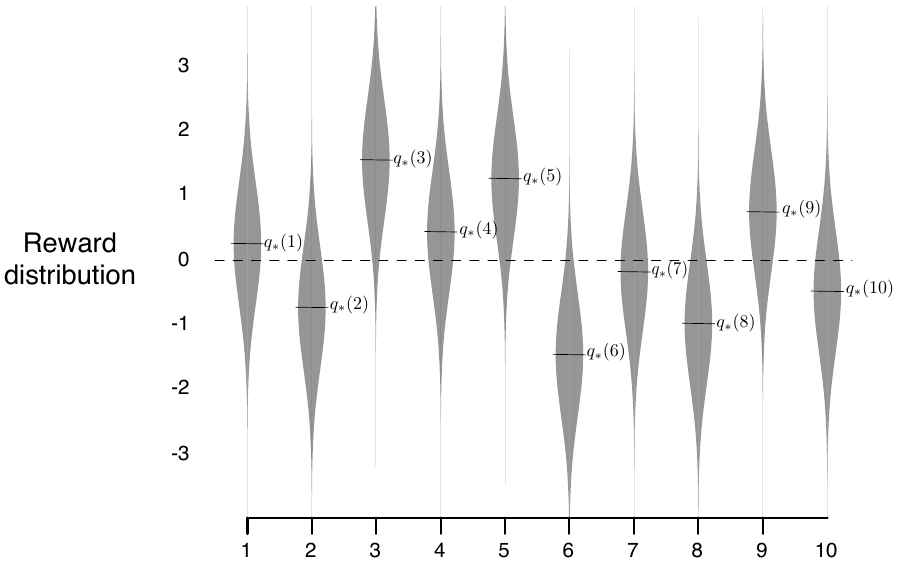
\includegraphics[width=0.9\textwidth]{figure-2-1.png}
\caption{10 臂测试平台中的一个赌博机问题示例。十个动作中每个动作的真实价值 $q_*(a)$，都从一个均值为零、单位方差的正态分布中选出；随后实际奖励从均值为 $q_*(a)$、单位方差的正态分布中选出，如这些灰色分布所示。}
\end{figure}

图 2.2 在 10 臂测试平台上比较了一种贪心方法和两种 $\varepsilon$-贪心方法（$\varepsilon=0.01$ 和 $\varepsilon=0.1$），它们正如上面所描述的那样。所有方法都使用样本平均技术来形成动作价值估计。上图显示期望奖励随着经验增长而增加。贪心方法在一开始比其他方法改进得稍快，但随后在较低水平处趋于平坦。在这个测试平台上，它每一步获得的奖励只有大约 1，而可能达到的最好值约为 1.55。贪心方法长期表现显著更差，因为它常常陷入执行次优动作。下图显示，贪心方法只在大约三分之一的任务中找到了最优动作。在另外三分之二的任务中，它对最优动作的初始采样令人失望，于是再也没有回到该动作。$\varepsilon$-贪心方法最终表现更好，因为它们持续探索，并提高了识别最优动作的机会。$\varepsilon=0.1$ 方法探索得更多，通常更早找到最优动作，但它选择该动作的时间比例从未超过 $91\%$。$\varepsilon=0.01$ 方法改进得较慢，但最终会在图中所示的两个性能度量上都优于 $\varepsilon=0.1$ 方法。也可以随时间减小 $\varepsilon$，试图同时获得较大值和较小值的优点。

\begin{figure}[htbp]
\centering
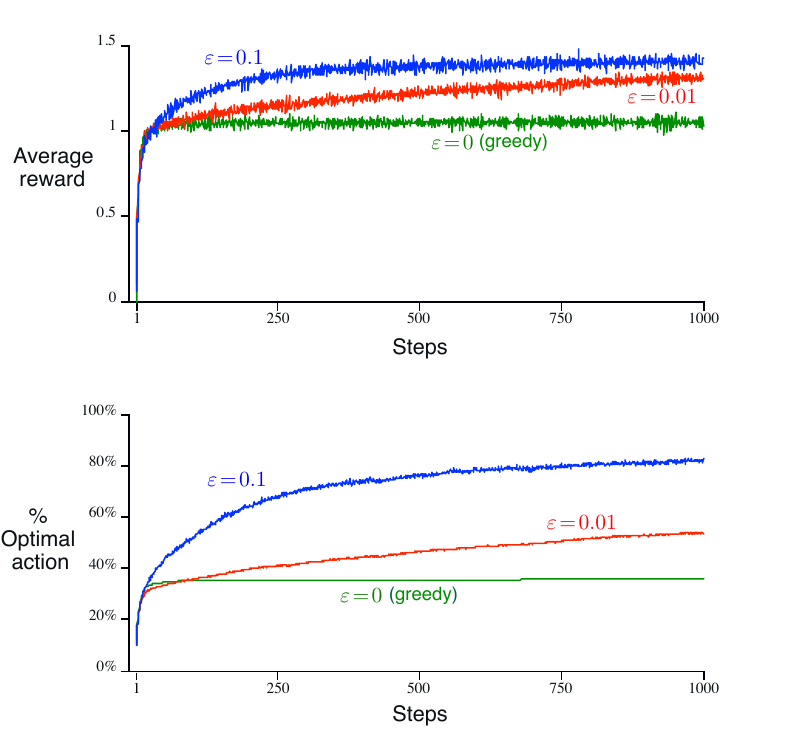
\includegraphics[width=0.82\textwidth]{figure-2-2.png}
\caption{10 臂测试平台上 $\varepsilon$-贪心动作价值方法的平均性能。这些数据是对 2000 次运行取平均得到的，每次运行使用不同的赌博机问题。所有方法都使用样本平均作为动作价值估计。}
\end{figure}

$\varepsilon$-贪心方法相对于贪心方法的优势依赖于任务。例如，假设奖励方差更大，比如是 10 而不是 1。面对噪声更大的奖励，需要更多探索才能找到最优动作，因而 $\varepsilon$-贪心方法相对于贪心方法应当表现得更好。另一方面，如果奖励方差为零，那么贪心方法在每个动作尝试一次之后就会知道它的真实价值。在这种情况下，贪心方法实际上可能表现最好，因为它会很快找到最优动作，然后再也不探索。但是，即使在确定性情形中，如果我们放宽其他某些假设，探索仍然会有很大优势。例如，假设赌博机任务是非平稳的，也就是说，动作的真实价值会随时间改变。在这种情况下，即使在确定性情形中，也需要探索，以确保某个非贪心动作没有变化到比贪心动作更好。正如我们将在接下来的几章中看到的，非平稳性是强化学习中最常遇到的情形。即使底层任务是平稳而确定性的，学习者也会面对一组类似赌博机的决策任务；随着学习的进行以及智能体决策策略的变化，这些任务中的每一个都会随时间改变。强化学习需要在探索与利用之间取得平衡。

\noindent\textbf{练习 2.2：赌博机示例}\quad 考虑一个 $k$ 臂赌博机问题，其中 $k=4$ 个动作，记为 1、2、3 和 4。考虑对这个问题应用一个使用 $\varepsilon$-贪心动作选择、样本平均动作价值估计、初始估计对所有 $a$ 都为 $Q_1(a)=0$ 的赌博机算法。假设初始的动作和奖励序列为 $A_1=1$，$R_1=-1$，$A_2=2$，$R_2=1$，$A_3=2$，$R_3=-2$，$A_4=2$，$R_4=2$，$A_5=3$，$R_5=0$。在这些时间步中的某些步，可能发生了 $\varepsilon$ 情形，从而导致随机选择动作。在哪些时间步这一定发生了？在哪些时间步这有可能发生？

\noindent\textbf{练习 2.3}\quad 在图 2.2 所示的比较中，从累积奖励和选择最佳动作的概率来看，哪一种方法在长期中表现最好？它会好多少？请定量表达你的答案。

\subsection*{2.4\quad 增量式实现}

到目前为止讨论的动作价值方法，都把动作价值估计为观察到的奖励的样本平均。现在我们转向这样一个问题：如何以计算上高效的方式计算这些平均值，特别是使用常数内存和常数的每时间步计算量。

为了简化记号，我们集中于单个动作。现在令 $R_i$ 表示第 $i$ 次选择\emph{这个动作}之后收到的奖励，并令 $Q_n$ 表示在它已经被选择 $n-1$ 次之后对其动作价值的估计；此时我们可以简单地写为
\[
Q_n\doteq \frac{R_1+R_2+\cdots+R_{n-1}}{n-1}.
\]
显然的实现方式，是维护所有奖励的记录，然后每当需要估计值时就执行这个计算。然而，如果这样做，那么随着看到的奖励越来越多，内存和计算需求会随时间增长。每一个额外奖励都需要额外内存来存储它，也需要额外计算来求分子中的和。

正如你可能猜到的，这其实并不必要。很容易设计出增量公式，用很小且固定的计算量来处理每个新奖励，从而更新平均值。给定 $Q_n$ 和第 $n$ 个奖励 $R_n$，所有 $n$ 个奖励的新平均值可以计算为
\begin{equation}
\begin{aligned}
Q_{n+1}
&= \frac{1}{n}\sum_{i=1}^{n}R_i\\
&= \frac{1}{n}\left(R_n+\sum_{i=1}^{n-1}R_i\right)\\
&= \frac{1}{n}\left(R_n+(n-1)\frac{1}{n-1}\sum_{i=1}^{n-1}R_i\right)\\
&= \frac{1}{n}\left(R_n+(n-1)Q_n\right)\\
&= \frac{1}{n}\left(R_n+nQ_n-Q_n\right)\\
&= Q_n+\frac{1}{n}\left[R_n-Q_n\right],
\end{aligned}
\tag{2.3}
\end{equation}
这个式子甚至在 $n=1$ 时也成立，此时对任意 $Q_1$ 都得到 $Q_2=R_1$。这种实现只需要为 $Q_n$ 和 $n$ 保留内存，并且对每个新奖励只需执行式（2.3）中的少量计算。

更新规则（2.3）具有一种在本书中反复出现的形式。一般形式是
\begin{equation}
\mathit{NewEstimate}\leftarrow \mathit{OldEstimate}
+\mathit{StepSize}\left[\mathit{Target}-\mathit{OldEstimate}\right].
\tag{2.4}
\end{equation}
表达式 $\left[\mathit{Target}-\mathit{OldEstimate}\right]$ 是估计中的一个\emph{误差}。通过朝“目标”方向迈出一步，这个误差被减小。目标被认为指出了一个值得移动的方向，虽然它可能带有噪声。在上面的情形中，例如，目标就是第 $n$ 个奖励。

注意，增量方法（2.3）中使用的步长参数（$\mathit{StepSize}$）会随时间步变化。在处理动作 $a$ 的第 $n$ 个奖励时，该方法使用步长参数 $\frac{1}{n}$。在本书中，我们用 $\alpha$ 表示步长参数，或者更一般地，用 $\alpha_t(a)$ 表示。

下面的框中给出了一个完整赌博机算法的伪代码，它使用增量计算的样本平均和 $\varepsilon$-贪心动作选择。函数 $\mathit{bandit}(a)$ 被假定为采取一个动作并返回相应奖励。

\begin{center}
\fbox{\begin{minipage}{0.86\textwidth}
\noindent\textbf{一个简单的赌博机算法}

\vspace{0.4em}
\noindent 初始化，对 $a=1$ 到 $k$：
\[
Q(a)\leftarrow 0,\qquad N(a)\leftarrow 0.
\]
\noindent 永远循环：
\[
A\leftarrow
\begin{cases}
\arg\max_a Q(a), & \text{以概率 }1-\varepsilon\text{（随机打破平局）},\\
\text{一个随机动作}, & \text{以概率 }\varepsilon,
\end{cases}
\]
\[
R\leftarrow \mathit{bandit}(A),\qquad
N(A)\leftarrow N(A)+1,
\]
\[
Q(A)\leftarrow Q(A)+\frac{1}{N(A)}\left[R-Q(A)\right].
\]
\end{minipage}}
\end{center}

\subsection*{2.5\quad 跟踪一个非平稳问题}

到目前为止讨论的平均方法适用于平稳赌博机问题，也就是说，适用于奖励概率不随时间改变的赌博机问题。如前所述，我们经常遇到实际上是非平稳的强化学习问题。在这种情况下，给予近期奖励比久远奖励更多权重是有意义的。做到这一点的最流行方式之一，是使用常数步长参数。例如，用于更新过去 $n-1$ 个奖励的平均值 $Q_n$ 的增量更新规则（2.3），可以修改为
\begin{equation}
Q_{n+1}\doteq Q_n+\alpha\left[R_n-Q_n\right],
\tag{2.5}
\end{equation}
其中步长参数 $\alpha\in(0,1]$ 是常数。这使得 $Q_{n+1}$ 成为过去奖励和初始估计 $Q_1$ 的加权平均：
\begin{equation}
\begin{aligned}
Q_{n+1}
&= Q_n+\alpha\left[R_n-Q_n\right]\\
&= \alpha R_n+(1-\alpha)Q_n\\
&= \alpha R_n+(1-\alpha)\left[\alpha R_{n-1}+(1-\alpha)Q_{n-1}\right]\\
&= \alpha R_n+(1-\alpha)\alpha R_{n-1}+(1-\alpha)^2Q_{n-1}\\
&= \alpha R_n+(1-\alpha)\alpha R_{n-1}+(1-\alpha)^2\alpha R_{n-2}\\
&\quad+\cdots+(1-\alpha)^{n-1}\alpha R_1+(1-\alpha)^nQ_1\\
&= (1-\alpha)^nQ_1+\sum_{i=1}^{n}\alpha(1-\alpha)^{n-i}R_i.
\end{aligned}
\tag{2.6}
\end{equation}
我们把它称为加权平均，是因为权重之和为
\[
(1-\alpha)^n+\sum_{i=1}^{n}\alpha(1-\alpha)^{n-i}=1,
\]
你可以自己验证这一点。注意，给予奖励 $R_i$ 的权重 $\alpha(1-\alpha)^{n-i}$ 依赖于它是在多少个奖励之前被观察到的，也就是 $n-i$。量 $1-\alpha$ 小于 1，因此，随着中间隔着的奖励数增加，给予 $R_i$ 的权重会减小。事实上，权重按照以 $1-\alpha$ 为底的指数方式衰减。（如果 $1-\alpha=0$，那么所有权重都放在最新奖励 $R_n$ 上，因为按照约定 $0^0=1$。）因此，这有时称为\emph{指数近因加权平均}。

有时让步长参数随时间步变化会很方便。令 $\alpha_n(a)$ 表示在处理第 $n$ 次选择动作 $a$ 之后收到的奖励时使用的步长参数。正如我们已经指出的，选择 $\alpha_n(a)=\frac{1}{n}$ 会得到样本平均方法；由大数定律，它保证收敛到真实动作价值。当然，并不是对序列 $\{\alpha_n(a)\}$ 的所有选择都保证收敛。随机逼近理论中的一个著名结果给出了以概率 1 保证收敛所需的条件：
\begin{equation}
\sum_{n=1}^{\infty}\alpha_n(a)=\infty
\quad\text{且}\quad
\sum_{n=1}^{\infty}\alpha_n^2(a)<\infty.
\tag{2.7}
\end{equation}
第一个条件用于保证步子足够大，从而最终克服任何初始条件或随机波动。第二个条件保证最终步子会变得足够小，从而确保收敛。

注意，在样本平均情形 $\alpha_n(a)=\frac{1}{n}$ 中，两个收敛条件都满足；但在常数步长参数情形 $\alpha_n(a)=\alpha$ 中并不满足。在后一种情形下，第二个条件不满足，这表明估计永远不会完全收敛，而是会随着最近收到的奖励继续变化。正如上面提到的，在非平稳环境中这实际上是可取的，而实际上非平稳的问题是强化学习中最常见的问题。此外，满足条件（2.7）的步长参数序列常常收敛很慢，或者需要相当多的调节才能获得令人满意的收敛速度。虽然满足这些收敛条件的步长参数序列常用于理论工作，但它们很少用于应用和经验研究。

\noindent\textbf{练习 2.4}\quad 如果步长参数 $\alpha_n$ 不是常数，那么估计 $Q_n$ 是先前收到的奖励的加权平均，但其权重不同于式（2.6）给出的权重。对于一般情形，与式（2.6）类似，用步长参数序列表示每个先前奖励上的权重是什么？

\noindent\textbf{练习 2.5（编程）}\quad 设计并实施一个实验，展示样本平均方法在非平稳问题上遇到的困难。使用 10 臂测试平台的一个修改版本，其中所有 $q_*(a)$ 一开始都相等，然后各自作独立随机游走（例如在每一步为所有 $q_*(a)$ 加上一个均值为零、标准差为 0.01 的正态分布增量）。绘制类似图 2.2 的图，一条曲线对应使用增量计算样本平均的动作价值方法，另一条曲线对应使用常数步长参数 $\alpha=0.1$ 的动作价值方法。使用 $\varepsilon=0.1$ 和更长的运行，例如 10000 步。

\subsection*{2.6\quad 乐观初始值}

到目前为止讨论的所有方法，都在某种程度上依赖于初始动作价值估计 $Q_1(a)$。用统计学的语言说，这些方法受到初始估计的\emph{偏置}。对于样本平均方法，一旦所有动作都至少被选择一次，偏置就会消失；但对于常数 $\alpha$ 的方法，偏置是永久的，虽然会按照式（2.6）随时间减小。在实践中，这种偏置通常不是问题，有时还会非常有用。缺点是初始估计实际上成为一组必须由使用者选择的参数，哪怕只是把它们全设为零。优点是，它们提供了一种简单方式，可以加入关于可期望奖励水平的某些先验知识。

初始动作价值也可以作为鼓励探索的一种简单方式。假设我们不把初始动作价值设为零，像在 10 臂测试平台中那样，而是把它们全设为 $+5$。回忆一下，在这个问题中，$q_*(a)$ 是从均值为 0、方差为 1 的正态分布中选出的。因此，初始估计 $+5$ 极其乐观。但这种乐观会鼓励动作价值方法探索。无论最初选择哪些动作，奖励都会低于起始估计；学习者会对所收到的奖励感到“失望”，于是转向其他动作。结果是，在价值估计收敛之前，所有动作都会被尝试若干次。即使始终选择贪心动作，系统也会进行相当数量的探索。

图 2.3 显示了在 10 臂赌博机测试平台上，使用 $Q_1(a)=+5$、对所有 $a$ 的贪心方法的性能。作为比较，图中还显示了一种 $\varepsilon$-贪心方法，它使用 $Q_1(a)=0$。最初，乐观方法表现较差，因为它探索得更多；但最终它表现更好，因为它的探索会随时间减少。我们把这种鼓励探索的技术称为\emph{乐观初始值}。我们认为它是一种简单技巧，在平稳问题上可能相当有效，但远不是一种一般有用的鼓励探索方法。例如，它并不很适合非平稳问题，因为它推动探索的力量本质上是暂时的。如果任务发生变化，产生了新的探索需求，这种方法帮不上忙。事实上，任何特别关注初始条件的方法，都不太可能有助于一般的非平稳情形。时间的开端只发生一次，因此我们不应过分关注它。这个批评同样适用于样本平均方法，因为它也把时间的开端当作一个特殊事件，以相等权重平均所有后续奖励。尽管如此，所有这些方法都很简单，其中一种方法，或者它们的某种简单组合，在实践中常常足够使用。在本书其余部分，我们会频繁使用这些简单探索技术中的几种。

\begin{figure}[htbp]
\centering
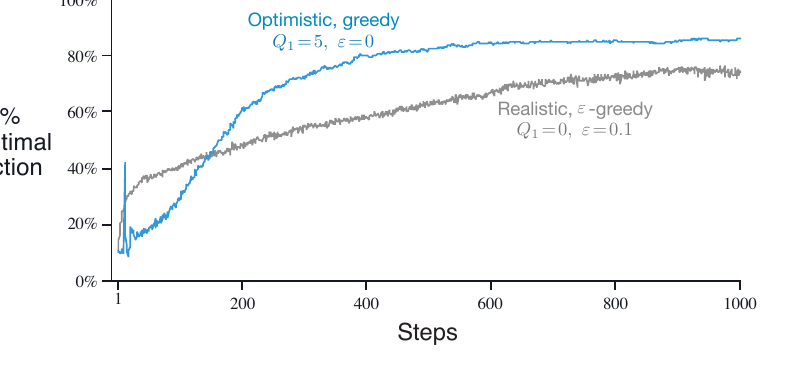
\includegraphics[width=0.82\textwidth]{figure-2-3.png}
\caption{乐观初始动作价值估计在 10 臂测试平台上的影响。两种方法都使用常数步长参数 $\alpha=0.1$。}
\end{figure}

\noindent\textbf{练习 2.6：神秘尖峰}\quad 图 2.3 中显示的结果应当相当可靠，因为它们是对 2000 个独立、随机选择的 10 臂赌博机任务取平均得到的。那么，为什么乐观方法曲线的早期部分会出现振荡和尖峰？换句话说，是什么可能使这种方法在某些早期步上平均表现得特别好或特别差？

\noindent\textbf{练习 2.7：无偏常数步长技巧}\quad 在本章的大部分内容中，我们使用样本平均来估计动作价值，因为样本平均不会产生常数步长所产生的那种初始偏置（见推导式（2.6）之前的分析）。然而，样本平均并不是一个完全令人满意的解法，因为它们在非平稳问题上可能表现很差。是否可能既避免常数步长的偏置，又保留它们在非平稳问题上的优势？一种方法是使用步长
\begin{equation}
\beta_n\doteq \alpha/\bar{o}_n,
\tag{2.8}
\end{equation}
来处理某个特定动作的第 $n$ 个奖励，其中 $\alpha>0$ 是一个常规的常数步长，而 $\bar{o}_n$ 是一个从 0 开始的迹：
\begin{equation}
\bar{o}_n\doteq \bar{o}_{n-1}+\alpha(1-\bar{o}_{n-1}),\quad n\ge 0,\quad \text{且 }\bar{o}_0\doteq 0.
\tag{2.9}
\end{equation}
作一个类似式（2.6）的分析，说明 $Q_n$ 是一个\emph{没有初始偏置}的指数近因加权平均。

\subsection*{2.7\quad 置信上界动作选择}

需要探索，是因为动作价值估计的准确性总是存在不确定性。贪心动作是目前看起来最好的动作，但其他某些动作实际上可能更好。$\varepsilon$-贪心动作选择迫使非贪心动作被尝试，但这种尝试没有区别对待，不会偏好那些几乎贪心或特别不确定的动作。更好的做法，是按照非贪心动作实际上可能为最优的潜力来选择它们，同时考虑它们的估计值离最大值有多近，以及这些估计中的不确定性。做到这一点的一种有效方式，是按照
\begin{equation}
A_t\doteq \arg\max_a\left[Q_t(a)+c\sqrt{\frac{\ln t}{N_t(a)}}\right],
\tag{2.10}
\end{equation}
来选择动作，其中 $\ln t$ 表示 $t$ 的自然对数（即为了等于 $t$，数 $e\approx2.71828$ 需要被提升到的幂），$N_t(a)$ 表示动作 $a$ 在时间 $t$ 之前被选择的次数（即式（2.1）中的分母），而数 $c>0$ 控制探索程度。如果 $N_t(a)=0$，那么认为 $a$ 是一个最大化动作。

这种\emph{置信上界}（upper confidence bound, UCB）动作选择的思想是，平方根项是对动作 $a$ 价值估计中不确定性或方差的度量。被最大化的量因此是动作 $a$ 可能真实价值的一种上界，其中 $c$ 决定置信水平。每次选择 $a$ 时，不确定性大概会降低：$N_t(a)$ 增加，而且由于它出现在分母中，不确定性项减小。另一方面，每次选择的不是动作 $a$ 时，$t$ 增加但 $N_t(a)$ 不增加；因为 $t$ 出现在分子中，不确定性估计增加。使用自然对数意味着这种增加会随时间变小，但没有上界；所有动作最终都会被选择，但价值估计较低的动作，或者已经被频繁选择的动作，会随时间以递减的频率被选择。

UCB 在 10 臂测试平台上的结果如图 2.4 所示。UCB 常常表现很好，正如此处所示；但与 $\varepsilon$-贪心相比，它更难从赌博机扩展到本书其余部分考虑的更一般强化学习设定。一个困难在于处理非平稳问题；这需要比第 2.5 节中介绍的方法更复杂的方法。另一个困难在于处理大的状态空间，特别是在使用本书第二部分所发展的函数近似时。在这些更高级的设定中，UCB 动作选择的思想通常并不实用。

\begin{figure}[htbp]
\centering
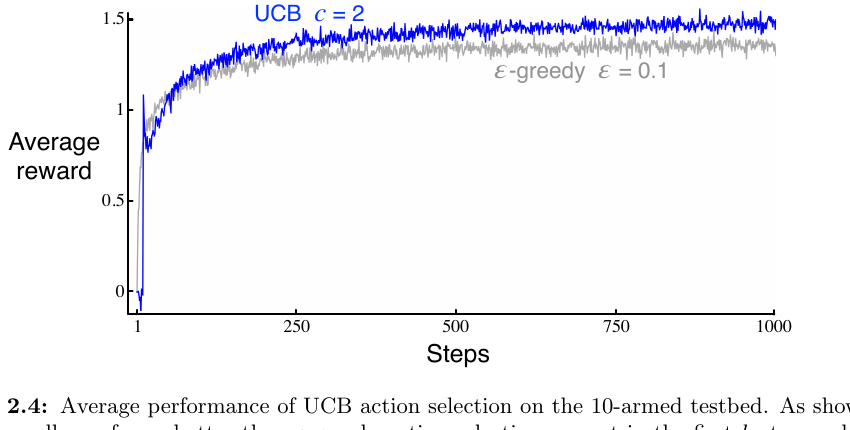
\includegraphics[width=0.82\textwidth]{figure-2-4.png}
\caption{10 臂测试平台上 UCB 动作选择的平均性能。如图所示，除了最初的 $k$ 步之外，UCB 通常比 $\varepsilon$-贪心动作选择表现更好；在最初的 $k$ 步中，它在尚未尝试的动作之间随机选择。}
\end{figure}

\noindent\textbf{练习 2.8：UCB 尖峰}\quad 在图 2.4 中，UCB 算法在第 11 步表现出一个明显的性能尖峰。为什么会这样？注意，要使你的答案完全令人满意，必须同时解释为什么奖励在第 11 步增加，以及为什么它在随后的步中下降。提示：如果 $c=1$，那么尖峰不那么明显。

\subsection*{2.8\quad 梯度赌博机算法}

到目前为止，在本章中我们考虑的是估计动作价值并用这些估计来选择动作的方法。这通常是一种好方法，但并不是唯一可能的方法。在本节中，我们考虑为每个动作 $a$ 学习一个数值\emph{偏好}，记为 $H_t(a)$。偏好越大，该动作被采取得越频繁；但偏好本身没有奖励意义上的解释。只有一个动作相对于另一个动作的相对偏好才重要：如果给所有动作偏好都加上 1000，对动作概率没有影响；动作概率按照如下的 \emph{soft-max} 分布（即 Gibbs 或 Boltzmann 分布）确定：
\begin{equation}
\Pr\{A_t=a\}\doteq
\frac{e^{H_t(a)}}{\sum_{b=1}^{k}e^{H_t(b)}}
\doteq \pi_t(a),
\tag{2.11}
\end{equation}
这里我们还引入了一个有用的新记号 $\pi_t(a)$，表示在时间 $t$ 采取动作 $a$ 的概率。最初所有动作偏好都相同（例如，对所有 $a$，$H_1(a)=0$），因此所有动作有相同的被选择概率。

\noindent\textbf{练习 2.9}\quad 说明在两个动作的情形下，soft-max 分布与统计学和人工神经网络中常用的 logistic 或 sigmoid 函数所给出的分布相同。

对于这一设定，有一种基于随机梯度上升思想的自然学习算法。在每一步，选择动作 $A_t$ 并收到奖励 $R_t$ 之后，动作偏好按如下方式更新：
\begin{equation}
\begin{aligned}
H_{t+1}(A_t)&\doteq H_t(A_t)+\alpha(R_t-\bar R_t)(1-\pi_t(A_t)),\\
H_{t+1}(a)&\doteq H_t(a)-\alpha(R_t-\bar R_t)\pi_t(a),\quad \text{对所有 }a\ne A_t,
\end{aligned}
\tag{2.12}
\end{equation}
其中 $\alpha>0$ 是步长参数，而 $\bar R_t\in\mathbb{R}$ 是直到并包括时间 $t$ 的所有奖励的平均值，它可以像第 2.4 节所述那样增量计算（如果问题是非平稳的，也可以像第 2.5 节那样计算）。$\bar R_t$ 项充当与奖励进行比较的基线。如果奖励高于基线，那么未来采取 $A_t$ 的概率增加；如果奖励低于基线，那么概率降低。未被选择的动作则朝相反方向移动。

图 2.5 显示了梯度赌博机算法在 10 臂测试平台一个变体上的结果；在这个变体中，真实期望奖励从一个均值为 $+4$ 而不是 0 的正态分布中选出（方差仍为 1）。由于奖励基线项会立即适应新的水平，所有奖励整体上移对梯度赌博机算法完全没有影响。但如果省略基线（也就是说，在式（2.12）中把 $\bar R_t$ 取为常数 0），那么性能会显著下降，如图中所示。

\begin{figure}[htbp]
\centering
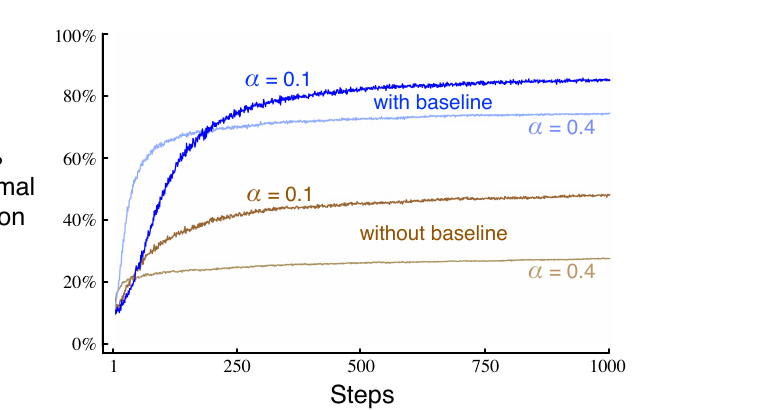
\includegraphics[width=0.82\textwidth]{figure-2-5.png}
\caption{当 $q_*(a)$ 被选为接近 $+4$ 而不是接近零时，在 10 臂测试平台上，带奖励基线和不带奖励基线的梯度赌博机算法的平均性能。}
\end{figure}

\noindent\textbf{作为随机梯度上升的赌博机梯度算法}

\vspace{0.4em}
通过把梯度赌博机算法理解为梯度上升的一种随机逼近，可以获得更深的见解。在精确的\emph{梯度上升}中，每个动作偏好 $H_t(a)$ 都会按照该增量对性能的影响成比例地增加：
\begin{equation}
H_{t+1}(a)\doteq H_t(a)+\alpha\frac{\partial \mathbb{E}[R_t]}{\partial H_t(a)},
\tag{2.13}
\end{equation}
这里的性能度量是期望奖励：
\[
\mathbb{E}[R_t]=\sum_x\pi_t(x)q_*(x),
\]
而增量影响的度量是这个性能度量关于动作偏好的偏导数。当然，在我们的情形中无法精确实现梯度上升，因为按假设我们不知道 $q_*(x)$；但实际上，我们算法（2.12）的更新在期望意义下等于式（2.13），从而该算法是随机梯度上升的一个实例。说明这一点的计算只需要初等微积分，但要分几步进行。

首先，我们更仔细地考察精确性能梯度：
\[
\begin{aligned}
\frac{\partial \mathbb{E}[R_t]}{\partial H_t(a)}
&= \frac{\partial}{\partial H_t(a)}\left[\sum_x\pi_t(x)q_*(x)\right]\\
&= \sum_x q_*(x)\frac{\partial \pi_t(x)}{\partial H_t(a)}\\
&= \sum_x \left(q_*(x)-B_t\right)\frac{\partial \pi_t(x)}{\partial H_t(a)},
\end{aligned}
\]
其中 $B_t$ 称为\emph{基线}，可以是不依赖于 $x$ 的任意标量。这里可以加入基线而不改变等式，因为梯度对所有动作求和为零，
\[
\sum_x \frac{\partial \pi_t(x)}{\partial H_t(a)}=0.
\]
当 $H_t(a)$ 改变时，有些动作的概率上升，有些动作的概率下降，但变化量之和必须为零，因为概率之和总是 1。

接下来，我们把求和中的每一项乘以 $\pi_t(x)/\pi_t(x)$：
\[
\frac{\partial \mathbb{E}[R_t]}{\partial H_t(a)}
=\sum_x \pi_t(x)\left(q_*(x)-B_t\right)
\frac{\partial \pi_t(x)}{\partial H_t(a)}/\pi_t(x).
\]
这个方程现在具有期望的形式：它对随机变量 $A_t$ 的所有可能取值 $x$ 求和，然后乘以取这些值的概率。因此，
\[
\begin{aligned}
&= \mathbb{E}\left[\left(q_*(A_t)-B_t\right)
\frac{\partial \pi_t(A_t)}{\partial H_t(a)}/\pi_t(A_t)\right]\\
&= \mathbb{E}\left[\left(R_t-\bar R_t\right)
\frac{\partial \pi_t(A_t)}{\partial H_t(a)}/\pi_t(A_t)\right],
\end{aligned}
\]
这里我们选择基线 $B_t=\bar R_t$，并用 $R_t$ 代替 $q_*(A_t)$，这是允许的，因为 $\mathbb{E}[R_t\mid A_t]=q_*(A_t)$。稍后我们将证明
\[
\frac{\partial \pi_t(x)}{\partial H_t(a)}
=\pi_t(x)\left(\mathbbm{1}_{a=x}-\pi_t(a)\right),
\]
其中 $\mathbbm{1}_{a=x}$ 定义为当 $a=x$ 时为 1，否则为 0。暂时假设这一点，则有
\[
\begin{aligned}
&= \mathbb{E}\left[\left(R_t-\bar R_t\right)
\pi_t(A_t)\left(\mathbbm{1}_{a=A_t}-\pi_t(a)\right)/\pi_t(A_t)\right]\\
&= \mathbb{E}\left[\left(R_t-\bar R_t\right)
\left(\mathbbm{1}_{a=A_t}-\pi_t(a)\right)\right].
\end{aligned}
\]
回忆一下，我们的计划是把性能梯度写成某个每一步都能采样的量的期望，正如刚才所做的那样，然后在每一步按照这个样本成比例地更新。把上面期望的一个样本代入式（2.13）中的性能梯度，得到
\[
H_{t+1}(a)=H_t(a)+\alpha(R_t-\bar R_t)
\left(\mathbbm{1}_{a=A_t}-\pi_t(a)\right),\quad \text{对所有 }a,
\]
你可以看出它等价于我们原来的算法（2.12）。

于是只剩下说明
\[
\frac{\partial \pi_t(x)}{\partial H_t(a)}
=\pi_t(x)\left(\mathbbm{1}_{a=x}-\pi_t(a)\right),
\]
正如我们所假定的。回忆导数的标准商法则：
\[
\frac{\partial}{\partial x}\left[\frac{f(x)}{g(x)}\right]
=\frac{\frac{\partial f(x)}{\partial x}g(x)-f(x)\frac{\partial g(x)}{\partial x}}{g(x)^2}.
\]
使用它，我们可以写出
\[
\begin{aligned}
\frac{\partial \pi_t(x)}{\partial H_t(a)}
&= \frac{\partial}{\partial H_t(a)}\pi_t(x)\\
&= \frac{\partial}{\partial H_t(a)}
\left[\frac{e^{H_t(x)}}{\sum_{y=1}^{k}e^{H_t(y)}}\right]\\
&= \frac{\frac{\partial e^{H_t(x)}}{\partial H_t(a)}\sum_{y=1}^{k}e^{H_t(y)}
-e^{H_t(x)}\frac{\partial \sum_{y=1}^{k}e^{H_t(y)}}{\partial H_t(a)}}
{\left(\sum_{y=1}^{k}e^{H_t(y)}\right)^2}\\
&= \frac{\mathbbm{1}_{a=x}e^{H_t(x)}\sum_{y=1}^{k}e^{H_t(y)}
-e^{H_t(x)}e^{H_t(a)}}
{\left(\sum_{y=1}^{k}e^{H_t(y)}\right)^2}\\
&= \frac{\mathbbm{1}_{a=x}e^{H_t(x)}}{\sum_{y=1}^{k}e^{H_t(y)}}
-\frac{e^{H_t(x)}e^{H_t(a)}}{\left(\sum_{y=1}^{k}e^{H_t(y)}\right)^2}\\
&= \mathbbm{1}_{a=x}\pi_t(x)-\pi_t(x)\pi_t(a)\\
&= \pi_t(x)\left(\mathbbm{1}_{a=x}-\pi_t(a)\right).
\end{aligned}
\]
我们刚刚说明了梯度赌博机算法的期望更新等于期望奖励的梯度，因此该算法是随机梯度上升的一个实例。这使我们确信该算法具有稳健的收敛性质。

注意，除了奖励基线不依赖于所选择的动作之外，我们并不要求它具有任何性质。例如，我们可以把它设为 0 或 1000，算法仍然是随机梯度上升的一个实例。基线的选择不影响算法的期望更新，但会影响更新的方差，因而影响收敛速度（例如如图 2.5 所示）。选择奖励平均值作为基线也许不是最优的，但它简单，并且在实践中效果很好。

\subsection*{2.9\quad 关联搜索（上下文赌博机）}

到目前为止，在本章中我们只考虑了非关联任务，也就是说，不需要把不同动作与不同情境关联起来的任务。在这些任务中，学习者要么在任务平稳时试图找到单个最佳动作，要么在任务非平稳时试图跟踪随时间变化的最佳动作。然而，在一般强化学习任务中，存在不止一个情境，目标是学习一个策略：把情境映射到在这些情境中最好的动作。为了为完整问题作铺垫，我们简要讨论非关联任务扩展到关联设定的最简单方式。

举一个例子，假设有若干不同的 $k$ 臂赌博机任务，并且在每一步你随机面对其中一个。因此，赌博机任务会从一步到下一步随机改变。对你而言，这看起来像一个单一的、非平稳的 $k$ 臂赌博机任务，其真实动作价值从一步到下一步随机改变。你可以尝试使用本章所描述的、能够处理非平稳性的方法之一；但除非真实动作价值变化很慢，否则这些方法效果不会很好。不过现在假设，当一个赌博机任务被选中给你时，你会得到关于其身份的一些可区分线索（但不是它的动作价值）。也许你面对的是一台真实老虎机，它在改变动作价值时会改变显示屏的颜色。现在你可以学习一个策略，把每个任务，也就是你看到的颜色，关联到面对该任务时应采取的最佳动作；例如，如果是红色就选择臂 1，如果是绿色就选择臂 2。若有正确策略，相比于没有任何信息来区分一个赌博机任务和另一个任务时，你通常可以做得好得多。

这是一个\emph{关联搜索}任务的例子；之所以这样称呼，是因为它既涉及通过试错学习来\emph{搜索}最佳动作，也涉及把这些动作与它们表现最好的情境\emph{关联}起来。在文献中，关联搜索任务现在常称为\emph{上下文赌博机}。关联搜索任务介于 $k$ 臂赌博机问题和完整强化学习问题之间。它们像完整强化学习问题一样涉及学习一个策略，但又像我们这个 $k$ 臂赌博机问题版本一样，每个动作只影响即时奖励。如果允许动作既影响\emph{下一个情境}又影响奖励，那么我们就得到完整强化学习问题。我们将在下一章提出这个问题，并在本书其余部分考察它的各种影响。

\noindent\textbf{练习 2.10}\quad 假设你面对一个 2 臂赌博机任务，它的真实动作价值会从一个时间步到下一个时间步随机改变。具体地说，假设在任意时间步，动作 1 和动作 2 的真实价值分别以概率 0.5 为 0.1 和 0.2（情形 A），并且以概率 0.5 为 0.9 和 0.8（情形 B）。如果你在任何时间步都不能判断自己面对的是哪种情形，那么你能达到的最佳成功期望是多少？应该如何行动才能达到它？现在假设在每一步都会告诉你正面对情形 A 还是情形 B（虽然你仍不知道真实动作价值）。这是一个关联搜索任务。在这个任务中你能达到的最佳成功期望是多少？应该如何行动才能达到它？

\subsection*{2.10\quad 小结}

本章提出了几种在探索与利用之间取得平衡的简单方式。$\varepsilon$-贪心方法在一小部分时间中随机选择，而 UCB 方法作确定性选择，但通过在每一步微妙地偏向到目前为止采样较少的动作来实现探索。梯度赌博机算法并不估计动作价值，而是估计动作偏好，并使用 soft-max 分布以分级的、概率性的方式偏向更受偏好的动作。简单而恰当地把初始估计设得乐观，甚至会使贪心方法也显著探索。

自然会问这些方法中哪一种最好。虽然一般而言这很难回答，但我们当然可以把它们全部运行在本章一直使用的 10 臂测试平台上，并比较它们的性能。一个复杂之处是，它们都有参数；为了得到有意义的比较，我们必须把它们的性能看作各自参数的函数来考察。到目前为止，我们的图展示了每种算法和参数设定随时间学习的过程，从而为该算法和参数设定产生一条\emph{学习曲线}。如果我们为所有算法和所有参数设定都绘制学习曲线，那么图会过于复杂拥挤，难以进行清楚比较。相反，我们用学习曲线在 1000 步上的平均值来概括一整条学习曲线；这个值正比于学习曲线下方的面积。图 2.6 显示了本章各种赌博机算法的这一度量，每种算法都作为它自身参数的函数，并在横轴上的单一尺度上显示。这种图称为\emph{参数研究}。注意，参数值按 2 倍因子变化，并以对数尺度呈现。还要注意每种算法性能的特征性倒 U 形；所有算法在其参数取中间值时表现最好，既不能太大也不能太小。在评估一种方法时，我们不仅应该关注它在最佳参数设定下表现得多好，还应该关注它对参数值有多敏感。所有这些算法都相当不敏感，在约一个数量级范围内变化的参数值上都表现良好。总体而言，在这个问题上，UCB 似乎表现最好。

\begin{figure}[htbp]
\centering
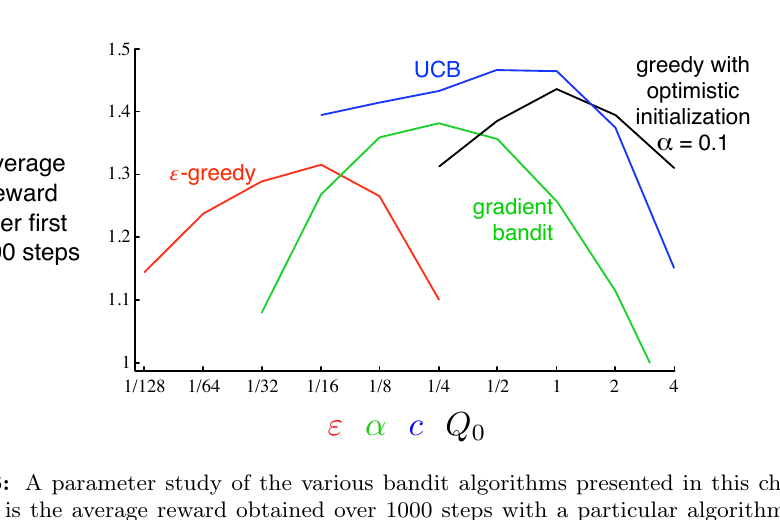
\includegraphics[width=0.82\textwidth]{figure-2-6.png}
\caption{本章介绍的各种赌博机算法的参数研究。每个点是在某个特定算法、某个特定参数设定下，1000 步内获得的平均奖励。}
\end{figure}

尽管这些方法很简单，但在我们看来，本章提出的方法已经相当可以看作当前水平。还有更复杂的方法，但它们的复杂性和假设使其不适用于我们真正关注的完整强化学习问题。从第 5 章开始，我们会提出求解完整强化学习问题的学习方法，其中会部分使用本章探索过的简单方法。

虽然本章探索的简单方法也许是目前能做的最好选择，但它们距离完全令人满意地解决探索与利用的平衡问题仍然很远。

在 $k$ 臂赌博机问题中，一种经过充分研究的平衡探索与利用的方法，是计算一种特殊动作价值，称为 \emph{Gittins 指数}。在某些重要的特殊情形中，这个计算是可处理的，并且会直接导向最优解；不过它确实需要完全知道可能问题的先验分布，而我们通常假定这种信息不可用。此外，无论是该方法的理论还是计算可处理性，看起来都不能推广到本书其余部分考虑的完整强化学习问题。

Gittins 指数方法是\emph{贝叶斯}方法的一个实例；贝叶斯方法假定动作价值上有一个已知的初始分布，然后在每一步之后精确更新该分布（假定真实动作价值是平稳的）。一般而言，更新计算可能非常复杂；但对于某些特殊分布（称为\emph{共轭先验}），它们很容易。一种可能性是，随后在每一步按照每个动作成为最佳动作的后验概率来选择动作。这种方法有时称为\emph{后验采样}或 \emph{Thompson 采样}，其表现常常类似于本章提出的无分布方法中最好的那些。

在贝叶斯设定中，甚至可以设想计算探索与利用之间的\emph{最优}平衡。对于任意可能动作，可以计算每种可能即时奖励的概率，以及由此得到的动作价值后验分布。这个演化中的分布成为问题的\emph{信息状态}。给定一个视界，例如 1000 步，我们可以考虑所有可能动作、所有可能产生的奖励、所有可能的下一动作、所有下一奖励，等等，一直到所有 1000 步。在给定假设下，每条可能事件链的奖励和概率都可以确定，然后只需选择最好的那一条。但可能性树增长得极快；即使只有两个动作和两个奖励，这棵树也会有 $2^{2000}$ 个叶子。通常不可行的是精确执行这种巨大计算，但也许可以有效近似。这种方法实际上会把赌博机问题变成完整强化学习问题的一个实例。最终，我们也许能够使用近似强化学习方法，例如本书第二部分介绍的方法，来逼近这个最优解。但这属于研究主题，超出了本导论性书籍的范围。

\noindent\textbf{练习 2.11（编程）}\quad 为练习 2.5 中概述的非平稳情形制作一张类似图 2.6 的图。包括常数步长的 $\varepsilon$-贪心算法，其中 $\alpha=0.1$。使用 200000 步的运行，并且对于每个算法和参数设定，以最后 100000 步的平均奖励作为性能度量。

\section*{书目与历史注记}

\noindent\textbf{2.1}\quad 赌博机问题已经在统计学、工程学和心理学中得到研究。在统计学中，赌博机问题属于“实验的序贯设计”这一主题；它由 Thompson（1933, 1934）和 Robbins（1952）引入，并由 Bellman（1956）研究。Berry 和 Fristedt（1985）从统计学视角对赌博机问题作了广泛处理。Narendra 和 Thathachar（1989）从工程学视角处理赌博机问题，并很好地讨论了围绕这些问题形成的各种理论传统。在心理学中，赌博机问题在统计学习理论中发挥过作用（例如 Bush 和 Mosteller，1955；Estes，1950）。

术语 greedy 常用于启发式搜索文献（例如 Pearl，1984）。探索与利用之间的冲突，在控制工程中被称为辨识（或估计）与控制之间的冲突（例如 Witten，1976b）。Feldbaum（1965）称其为\emph{双重控制}问题，指的是在不确定性下试图控制系统时，需要同时求解辨识和控制这两个问题。在讨论遗传算法的某些方面时，Holland（1975）强调了这种冲突的重要性，称其为利用的需要与新信息的需要之间的冲突。

\noindent\textbf{2.2}\quad 我们的 $k$ 臂赌博机问题的动作价值方法，最早由 Thathachar 和 Sastry（1985）提出。在学习自动机文献中，这些方法常称为估计器算法。术语 action value 归功于 Watkins（1989）。最早使用 $\varepsilon$-贪心方法的也可能是 Watkins（1989，第 187 页），但这个想法很简单，因此似乎很可能早已有所使用。

\noindent\textbf{2.4--5}\quad 这些材料属于随机迭代算法的一般主题，Bertsekas 和 Tsitsiklis（1996）对此有很好的覆盖。

\noindent\textbf{2.6}\quad Sutton（1996）在强化学习中使用了乐观初始化。

\noindent\textbf{2.7}\quad 使用置信上界估计来选择动作的早期工作由 Lai 和 Robbins（1985）、Kaelbling（1993b）以及 Agrawal（1995）完成。这里提出的 UCB 算法在文献中称为 UCB1，最早由 Auer、Cesa-Bianchi 和 Fischer（2002）发展出来。

\noindent\textbf{2.8}\quad 梯度赌博机算法是 Williams（1992）引入的基于梯度的强化学习算法的一个特例，后来发展成 actor--critic 算法和策略梯度算法；本书后面会讨论这些算法。我们这里的发展受到 Balaraman Ravindran（个人交流）的影响。关于基线选择的进一步讨论见该处，以及 Greensmith、Bartlett 和 Baxter（2002, 2004）及 Dick（2015）。类似算法的早期系统研究由 Sutton（1984）完成。

动作选择规则（2.11）的术语 soft-max 归功于 Bridle（1990）。该规则似乎最早由 Luce（1959）提出。

\noindent\textbf{2.9}\quad 术语 associative search 及相应问题由 Barto、Sutton 和 Brouwer（1981）引入。术语 associative reinforcement learning 也被用于关联搜索（Barto 和 Anandan，1985），但我们倾向于把这个术语保留为完整强化学习问题的同义词（如 Sutton，1984）。（并且，如我们所指出，现代文献也用“contextual bandits”这个术语称呼这个问题。）我们注意到，Thorndike 的效果律（第 1 章中引用）通过指称情境（状态）和动作之间关联链接的形成来描述关联搜索。按照操作性或工具性条件反射的术语（例如 Skinner，1938），辨别刺激是一种信号，表示某个特定强化依存关系存在。在我们的术语中，不同的辨别刺激对应不同的状态。

\noindent\textbf{2.10}\quad Bellman（1956）最早说明了如何在问题的贝叶斯表述中使用动态规划来计算探索与利用之间的最优平衡。Gittins 指数方法归功于 Gittins 和 Jones（1974）。Duff（1995）说明了如何通过强化学习来学习赌博机问题的 Gittins 指数。Kumar（1985）的综述很好地讨论了这些问题的贝叶斯和非贝叶斯方法。术语 information state 来自部分可观测 MDP 的文献；参见例如 Lovejoy（1991）。

其他理论研究关注探索效率，通常表述为算法能够多快接近最优决策策略。形式化探索效率的一种方式，是把监督学习算法的\emph{样本复杂度}概念适配到强化学习中；样本复杂度指算法为了在学习目标函数时达到所需准确度而需要的训练样本数。强化学习算法的探索样本复杂度的一个定义，是算法没有选择近似最优动作的时间步数（Kakade，2003）。Li（2012）在一篇关于强化学习中探索效率理论方法的综述中讨论了这一点以及其他若干方法。Russo、Van Roy、Kazerouni、Osband 和 Wen（2018）提供了 Thompson 采样的详尽现代处理。

\end{document}
